\documentclass[14pt]{article}
\usepackage
[
        a4paper,% other options: a3paper, a5paper, etc
        left=2cm,
        right=2cm,
        top=3cm,
        bottom=4cm,
]
{geometry}

\usepackage[utf8]{inputenc}
\usepackage{listings}
\usepackage{xcolor}
\usepackage{graphicx}
\lstset { %
    language=C++,
    backgroundcolor=\color{black!5}, % set backgroundcolor
    basicstyle=\footnotesize,% basic font setting
}


\title{Report.1.OpenMP}
\author{lehuyduc3 }
\date{November 2020}
\usepackage{indentfirst}
\parindent{}

\begin{document}

\maketitle

\section{How to implement OpenMP parallel-loop}
Just add
\begin{verbatim}
    #pragma omp parallel for
\end{verbatim}
before the inner loop.

\begin{lstlisting}
for (int j = 0; j < 100; j++) {     // let's do it 100 times, otherwise it's too fast!
            #pragma omp parallel for
            for (int i = 0; i < pixelCount; i++) {
                outputImage[i * 3] = (char) (((int) inputImage->buffer[i * 3] 
                                            + (int) inputImage->buffer[i * 3 + 1] +
                                            (int) inputImage->buffer[i * 3 + 2]) / 3);
                outputImage[i * 3 + 1] = outputImage[i * 3];
                outputImage[i * 3 + 2] = outputImage[i * 3];
            }
        }
\end{lstlisting}

\section{Speedup and effects of parameters}
\subsection{Team size}

\begin{figure}[h]
\centering
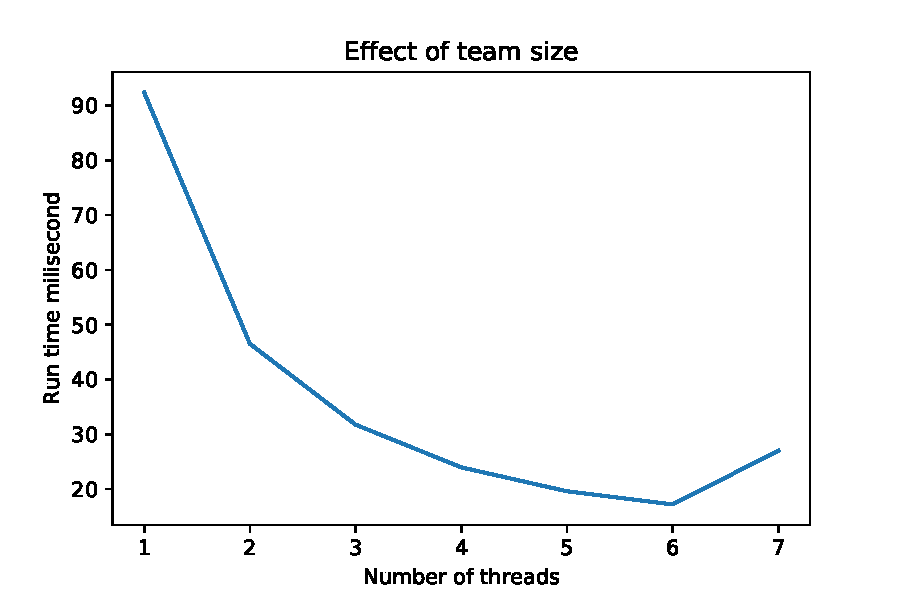
\includegraphics[scale=0.75]{report1_teamsize.pdf}
\end{figure}

Specs: i7-8750H, 6 cores 12 threads
We easily see that more thread = better, until there are more threads than actual cores.

\subsection{Dynamic schedule}
To test this, we divide the array (list of pixels) into small blocks. We use the size of each block as the "chunk" for the dynamic schedule. We use 6 threads for this benchmark.

\begin{figure}[h]
\centering
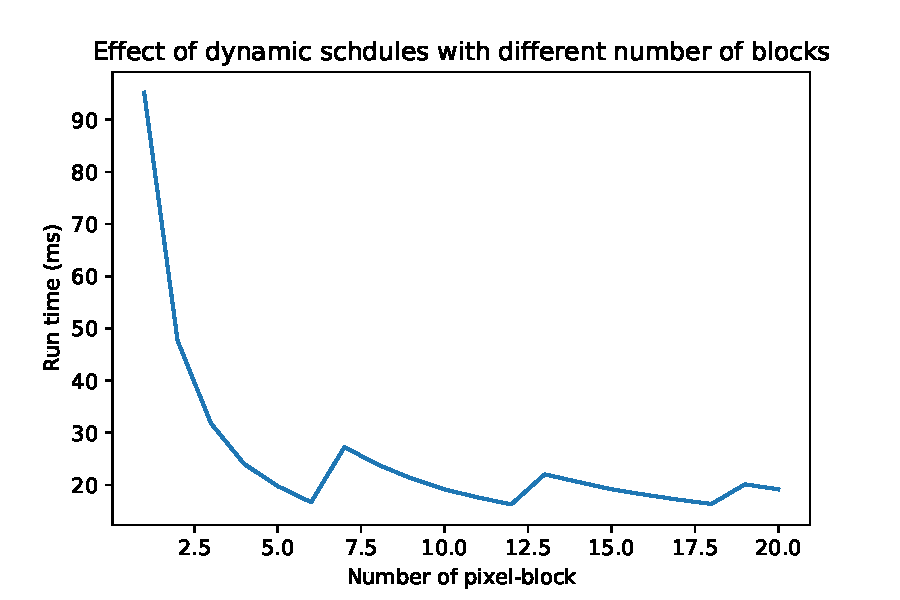
\includegraphics[scale=0.75]{report1_dynamic_schedule.pdf}
\end{figure}

The special thing here is that the running time is lowest when the number of blocks equals to multiples of 6 (6, 12, 18). This is because in that situation, the jobs are divided equally.
\end{document}
